\documentclass[problem]{mcs}

\begin{pcomments}
    \pcomment{TP_Faces_of_a_Planar_Embedding}
    \pcomment{Converted from planar-faces.scm by scmtotex and dmj
              on Sat 12 Jun 2010 09:38:41 PM EDT}
\end{pcomments}

\begin{problem}

%% type: short-answer
%% title: Faces of a Planar Embedding

What are the discrete faces of the following two graphs?
     
Write each cycle as a sequence of letters without spaces, starting
with the alphabetically earliest letter in the clockwise direction,
for example ``\STR{adbfa}.''  Separate the sequences with spaces.

\bparts

\ppart\leavevmode

\begin{center}
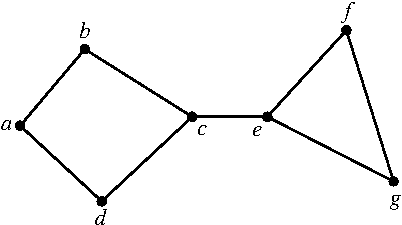
\includegraphics[height=1in]{edge-twice-same-face}
\end{center}

\begin{solution}

abcda, efge, abcefgecda

Don't forget the ``outside'' face.
\end{solution}

\ppart\leavevmode

\begin{center}
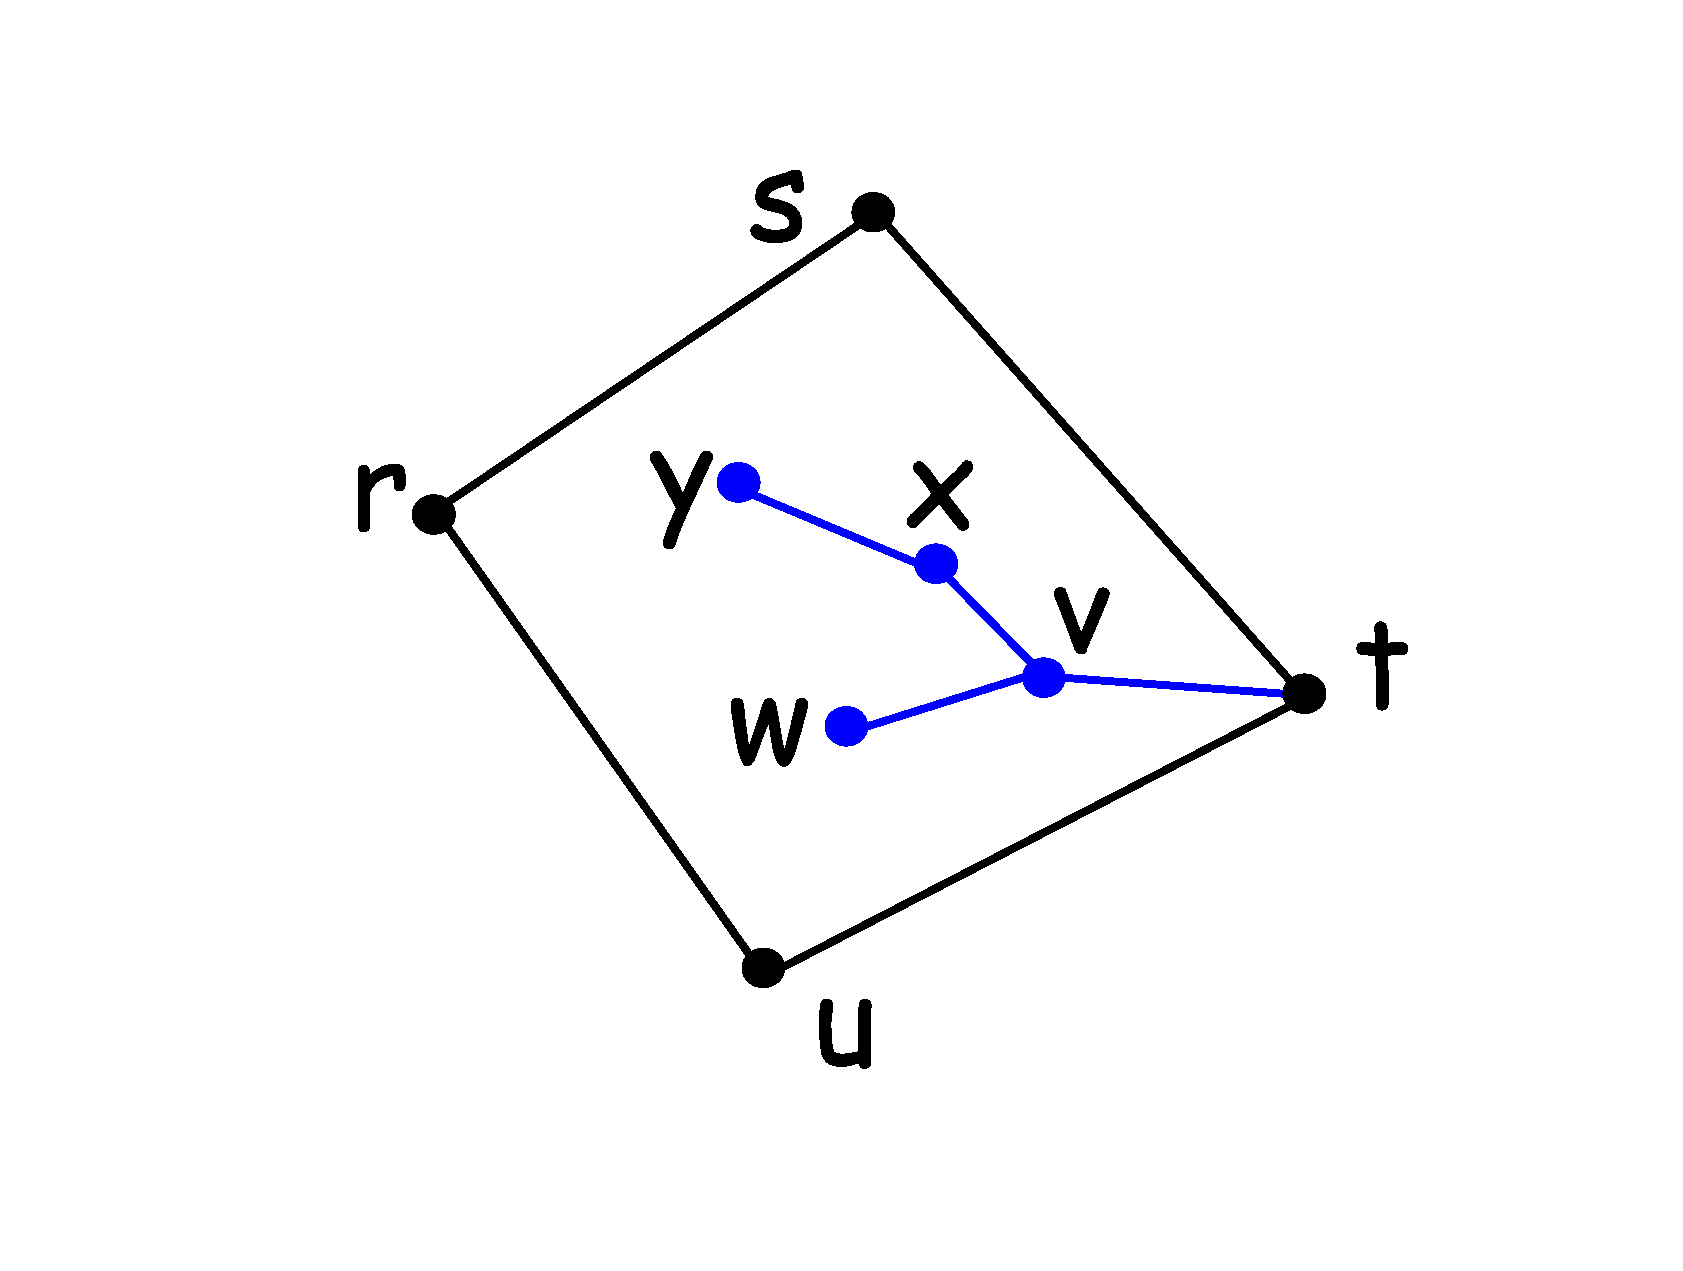
\includegraphics[height=1in]{dongle-face}
\end{center}

\begin{solution}

rstvwvxyxvtur,
rstur,
rstvxyxvwvtur,
rstur
\end{solution}

\eparts

\end{problem}

\endinput
